\chapter{Wstęp}
\section{Wprowadzenie}

Algorytmy automatycznej kontroli głośności (ang. automatic gain control - AGC) są elementem współczesnych systemów przetwarzania sygnałów zarówno akustycznych tak jak w poniższej pracy jak i na przykład radiowych \cite{agc_5g}. Celem stosowania takiego algorytmu w przypadku sygnałów akustycznych jest utrzymanie stałej głośności wszystkich mówców w danym systemie. Konkretnym przykładem zastosowania są wideokonferencje \cite{agc_application}, które z uwagi na sytację pandemiczną na świecie zyskały ogromną popularność. Z uwagi na różne czułości mikrofonów uczestników, różną głośność mówienia i odległość od mikrofonu, uczestnicy mogą odczuwać nieprzyjemne dla ucha fluktuacje głośności. Algorytm AGC redukuje te efekty. Ważne jest aby takie algorytmy skutkowały wysokim poziomem sygnału do szumu (ang. signal to noise ratio - SNR) jak i wysokim stosunkiem sygnału do pozostałych interferencji.

Najprostszym rozwiązaniem jest zastosowanie systemu jednokanałowego \cite{Archibald2008}. W takim systemie możlie jest tylko sterowanie głośnością sygnału wejściowego jako całości, na podstawie chwilowej wartości obwiedni. Uniemożliwia on jednak różny poziom wzmocnienia dla różnych mówców i usunięcie interferencji, jeśli współistnieją one w czasie z głównym sygnałem.

Rozwiązaniem bardziej skomplikowanym, zarówno od strony sprzętowej, programistycznej i czasu obliczeń jest użycie systemu z wieloma mikrofonami. Taki system umożliwia pożądane rozróżnienie między mówcami i eliminację interferencji \cite{Thiergart2013}. W systemie takim możliwa jest estymacja kierunków nadchodzenia fali, a co za tym idzie mocy nadchodzącej z wybranych stron i zastosowanie odpowiednich filtrów, które wzmacniają sygnał z żądanych kierunków.

W tej pracy skupiono się właśnie na drugim z wymienionych rodzajów algorytmów AGC. W pracy zostanie przedstawiona praktyczna implementacja bazująca na nagraniach z macierzy mikrofonowych.

\begin{figure}[h]
    \centering
    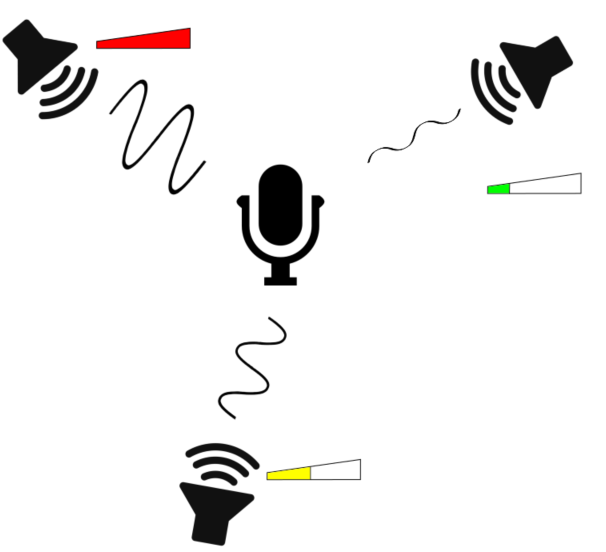
\includegraphics[width=\textwidth]{Images/setup.png}
    \caption{Graficzna reprezentacja problemu}
    \label{fig:setup}
\end{figure}

\section{Cel}
Celem pracy inżynierskiej była praktyczna implementacja istniejącego algorytmu AGC z tłumieniem tła akustycznego, wraz z estymacją kierunku nadchodzenia fali. Wybrany algorytm powinien spełniać cechy wymienione w poprzedniej sekcji, tj. pozwalać na regulację głośności nagrania osobno dla różnych mówców i minimalizować zakłócenia. Z tego powodu zdecydowano się na użycie tak zwanego filtra LCMV (ang. linearly constrained minimum variance). Opracowany algorytm w założeniu nie musi być algorytmem czasu rzeczywistego. Powinien wykonywać żądane operacje bazując na nagraniach z macierzy mikrofonowej. Kolejnym celem projektu było przeprowadzenie testów skuteczności zaimplementowanego systemu w różnych wariantach i warunkach pracy. W tym celu powstanie generator symulujący różne możliwe konfiguracje.

\section{Zakres wykonanej pracy}
Pierwszym z etapów pracy inżynierskiej było zapoznanie się autora pracy z dostępnymi publikacjami opisującymi zarówno tematykę AGC \cite{Braun2014}, \cite{Archibald2008} jak i generalną tematykę przetwarzania sygnałów dla macierzy czujników akustycznych \cite{Benesty2008} i wybór metody. Wybrana metoda bazuje w głównej mierze na metodzie \cite{Braun2014}.
Następnie dokonany został wybór środowiska pracy- języka Python wraz z paczką NumPy \cite{numpy}. Szczegółowy opis użytych narzędzie znajduje się w rodziale \ref{chapter-4}. Następnie autor pracy napisał symulator umożliwiający generację sygnałów mikrofonowych. Dalsza część realizacji pracy obejmowała- zaplanowanie praktycznej implementacji systemu, wykonanie tej implementacji i testy przy użyciu sygnałów macierzy mikrofonowej otrzymanej z symulatora. W testach skupiono się na ewaulacji systemu pod kątem działania dla jednego mówcy i wielu mówców. Sprawdzono odporność na zakłócenia i wpływ geometrii macierzy czujników akustycznych na działania poszczególnych składowych algorytmu.

